\documentclass[
11pt, % The default document font size, options: 10pt, 11pt, 12pt
%codirector, % Uncomment to add a codirector to the title page
]{charter} 




% El títulos de la memoria, se usa en la carátula y se puede usar el cualquier lugar del documento con el comando \ttitle
\titulo{Programador remoto de equipos electrónicos} 

% Nombre del posgrado, se usa en la carátula y se puede usar el cualquier lugar del documento con el comando \degreename
\posgrado{Carrera de Especialización en Sistemas Embebidos} 
%\posgrado{Carrera de Especialización en Internet de las Cosas} 
%\posgrado{Carrera de Especialización en Intelegencia Artificial}
%\posgrado{Maestría en Sistemas Embebidos} 
%\posgrado{Maestría en Internet de las cosas}

% Tu nombre, se puede usar el cualquier lugar del documento con el comando \authorname
\autor{Ing. José Mendoza} 

% El nombre del director y co-director, se puede usar el cualquier lugar del documento con el comando \supname y \cosupname y \pertesupname y \pertecosupname
\director{Mg. Ing. Sergio Starkloff}
\pertenenciaDirector{SURiX S.R.L} 
% FIXME:NO IMPLEMENTADO EL CODIRECTOR ni su pertenencia
\codirector{John Doe} % para que aparezca en la portada se debe descomentar la opción codirector en el documentclass
\pertenenciaCoDirector{FIUBA}

% Nombre del cliente, quien va a aprobar los resultados del proyecto, se puede usar con el comando \clientename y \empclientename
\cliente{Mg. Ing. Sergio Starkloff}
\empresaCliente{SURiX S.R.L}

% Nombre y pertenencia de los jurados, se pueden usar el cualquier lugar del documento con el comando \jurunoname, \jurdosname y \jurtresname y \perteunoname, \pertedosname y \pertetresname.
\juradoUno{Nombre y Apellido (1)}
\pertenenciaJurUno{pertenencia (1)} 
\juradoDos{Nombre y Apellido (2)}
\pertenenciaJurDos{pertenencia (2)}
\juradoTres{Nombre y Apellido (3)}
\pertenenciaJurTres{pertenencia (3)}
 
\fechaINICIO{22 de agosto de 2023}		%Fecha de inicio de la cursada de GdP \fechaInicioName
\fechaFINALPlan{10 de octubre de 2023} 	%Fecha de final de cursada de GdP
\fechaFINALTrabajo{10 de junio de 2024}	%Fecha de defensa pública del trabajo final


\begin{document}

\maketitle
\thispagestyle{empty}
\pagebreak


\thispagestyle{empty}
{\setlength{\parskip}{0pt}
\tableofcontents{}
}
\pagebreak


\section*{Registros de cambios}
\label{sec:registro}


\begin{table}[ht]
\label{tab:registro}
\centering
\begin{tabularx}{\linewidth}{@{}|c|X|c|@{}}
\hline
\rowcolor[HTML]{C0C0C0} 
Revisión & \multicolumn{1}{c|}{\cellcolor[HTML]{C0C0C0}Detalles de los cambios realizados} & Fecha      \\ \hline
v1.0      & Creación del documento                                 &\fechaInicioName \\ \hline
%1      & Se completa hasta el punto 4 inclusive                 & dd/mm/aaaa \\ \hline
v2.0      & Se completa hasta el punto 9				& 28 de septiembre de 2023 \\ \hline
%		  Se puede agregar algo más \newline
%		  En distintas líneas \newline
%		  Así                                                    & dd/mm/aaaa \\ \hline
v3.0      & Se completa hasta el punto 12                & 02 de octubre de 2023 \\ \hline
v4.0      & Se completa el plan	                                 & 03 de octubre de 2023 \\ \hline
\end{tabularx}
\end{table}

\pagebreak



\section*{Acta de constitución del proyecto}
\label{sec:acta}

\begin{flushright}
Buenos Aires, \fechaInicioName
\end{flushright}

\vspace{2cm}

Por medio de la presente se acuerda con el Ing. \authorname\hspace{1px} que su Trabajo Final de la \degreename\hspace{1px} se titulará ``\ttitle'', consistirá esencialmente en la implementación de un sistema que programe placas electrónicas mediante protocolo RS-232 y que los archivos de programación sean descargados por Wi-Fi y esos archivos podrán ser consultados a través de una página web, y tendrá un presupuesto preliminar estimado de 671 hs de trabajo, con fecha de inicio \fechaInicioName\hspace{1px} y fecha de presentación pública \fechaFinalName.

Se adjunta a esta acta la planificación inicial.

\vfill

% Esta parte se construye sola con la información que hayan cargado en el preámbulo del documento y no debe modificarla
\begin{table}[ht]
\centering
\begin{tabular}{ccc}
\begin{tabular}[c]{@{}c@{}}Dr. Ing. Ariel Lutenberg \\ Director posgrado FIUBA\end{tabular} & \hspace{2cm} & \begin{tabular}[c]{@{}c@{}}\clientename \\ \empclientename \end{tabular} \vspace{2.5cm} \\ 
\multicolumn{3}{c}{\begin{tabular}[c]{@{}c@{}} \supname \\ Director del Trabajo Final\end{tabular}} \vspace{2.5cm} \\
%\begin{tabular}[c]{@{}c@{}}\jurunoname \\ Jurado del Trabajo Final\end{tabular}     &  & \begin{tabular}[c]{@{}c@{}}\jurdosname\\ Jurado del Trabajo Final\end{tabular}  \vspace{2.5cm}  \\
%\multicolumn{3}{c}{\begin{tabular}[c]{@{}c@{}} \jurtresname\\ Jurado del Trabajo Final\end{tabular}} \vspace{.5cm}                                                                     
\end{tabular}
\end{table}




\section{1. Descripción técnica-conceptual del proyecto a realizar}
\label{sec:descripcion}


%\begin{consigna}{red} % El bloque "consigna" se usa para poner texto en rojo y dar una pequeña ayuda sobre cómo completar la sección. En cada entrega parcial deben eliminar los comandos begin y end del bloque consigna de las secciones que hayan completado.

El presente proyecto es realizado para la empresa SURiX. La empresa tiene un campo de actividad el cual es el desarrollo de productos que incluyan el protocolo IP, tales como portería, controles de acceso y anunciamientos.

La problemática actuál consiste en que la empresa tiene algunos productos (como controles de acceso) que solamente contemplan una interfaz de comunicación RS-232 para poder ser descargada una configuración.

La propuesta de proyecto consiste en diseñar un programador remoto que pueda cargar y descargar alguna configuración a un producto en específico mediante una interfaz de comunicación RS-232 y/o RS-285. Tal programador tendrá una conexión a internet mediante protocolo Wi-Fi para poder cargar y/o descargar los archivos de configuración. Estos archivos de configuración descargados por la placa conectada a internet serán descargados al control de acceso mediante una interfaz RS-232. De este modo se podrá actualizar los productos de SURiX de una forma remota. 

Además de los requerimientos anteriores, se diseñará una página web la cual interactuará con el servidor, enviándole comandos al programador remoto. Esta página web deberá ser capaz de cargar un archivo de configuración al servidor para que el programador remoto a diseñar pueda descargarlo o viceversa. Descargar un archivo de configuración que el programador remoto haya subido al servidor.
Por esto anterior se puede resumir el proyecto en unos puntos:

\begin{itemize}
	\item El proyecto es parte del programa de vinculación. Este proyecto será realizado para la empresa SURiX S.R.L.
	\item No existe algún tipo de financiamiento por parte de la empresa y tampoco hay un acuerdo de confidencialidad.
	\item El programador remoto a diseñar requiere de una conexión a internet mediante Wi-Fi o Ethernet.
	\item Se tendrá que diseñar una página web que servirá para almacenar el archivo de configuración el cual el programador remoto podrá descargar por Wi-Fi.
\end{itemize}



\begin{figure}[htpb]
\centering 
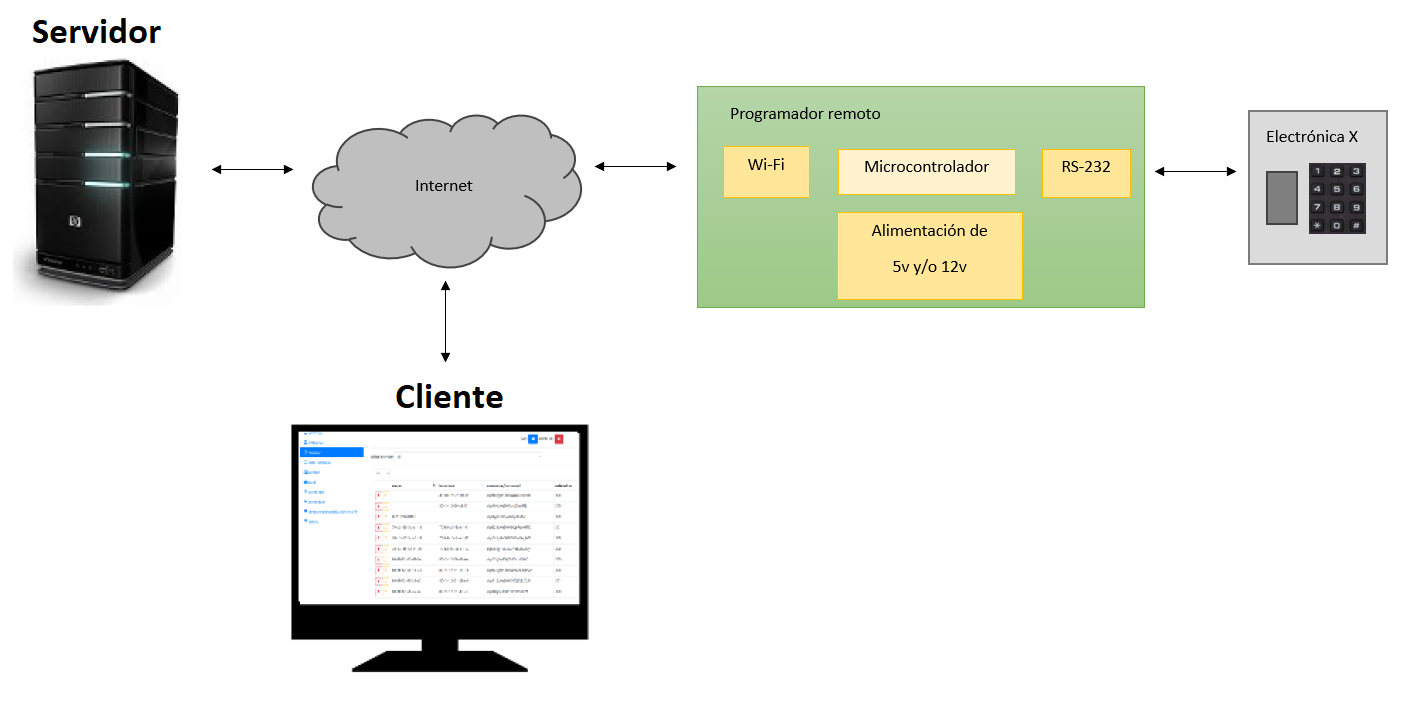
\includegraphics[width=1\textwidth]{./Figuras/DiagBloquesProgramador.png}
\caption{Diagrama en bloques del sistema}
\label{fig:diagBloques}
\end{figure}

\vspace{25px}

%\end{consigna}

\section{2. Identificación y análisis de los interesados}
\label{sec:interesados}


\begin{table}[ht]
%\caption{Identificación de los interesados}
%\label{tab:interesados}
\begin{tabularx}{\linewidth}{@{}|l|X|X|l|@{}}
\hline
\rowcolor[HTML]{C0C0C0} 
Rol           & Nombre y Apellido & Organización 	& Puesto 	\\ \hline
Cliente       & \clientename      &\empclientename	& Socio - Propietario \\ \hline
Responsable   & \authorname       & FIUBA        	& Alumno 	\\ \hline
Orientador    & \supname	      & \pertesupname 	& Director Trabajo final \\ \hline
Usuario final & Clientes de SURiX &       -      	&     -   	\\ \hline
\end{tabularx}
\end{table}



\begin{itemize}
	\item Cliente: Sergio Starkloff fue el que propuso el proyecto. Las reuniones con él son virtuales debido a que se encuentra fuera del país. En este proyecto también emplea el papel de Director.
	%\item Equipo: Juan Perez, suele pedir licencia porque tiene un familiar con una enfermedad. Planificar considerando esto.
	\item Orientador: Sergio Starkloff es también el orientador del proyecto. Cualquier duda técnica se le puede realizar a él.
	\item Usuario final: Los usuarios finales son los clientes de SURiX S.R.L que se ven en la necesidad de actualizar los productos de una forma remota.
\end{itemize}




\section{3. Propósito del proyecto}
\label{sec:proposito}


El propósito de este proyecto es desarrollar un programador remoto de equipos electrónicos . Este desarrollo permite poder cargar y descargar un archivo de configuracion a un servidor y además se desarrollará una página web en la que se podrá cargar los archivos de configuración que serán descargados al programador remoto.


\newpage
\section{4. Alcance del proyecto}
\label{sec:alcance}

Para la realización del presente trabajo se incluyen las siguientes actividades:

\begin{itemize}
	\item Investigación y elección del hardware (microcontrolador) a utilizar.
	\item Diseño y desarrollo de página web para la carga y descarga de archivos de configuración.
	\item Investigación sobre comunicación FTP para la carga y descarga de archivos desde el servidor.
\end{itemize}

El presente proyecto no incluye:

\begin{itemize}
	\item Diseño de algún chasis que proteja físicamente la placa vinculada al proyecto.
	\item Algún diseño de circuito de protección de alimentación hacia la placa.
\end{itemize}


\section{5. Supuestos del proyecto}
\label{sec:supuestos}


Para el desarrollo del presente proyecto se supone que:

\begin{itemize}
	\item Se contará con una placa ESP32 para el desarrollo del proyecto.
	\item El tiempo de desarrollo del proyecto es ajustado a la duración de la especialidad.
	 \item Se diseñará una página web para la carga y descarga de archivos al servidor.
	 \item El cliente pondrá el servidor en el cual se almacenará la página web y los archivos de configuración.
	 \item Las pruebas del prototipo se realizarán en un servidor local ya el producto final estará en el servidor del cliente.
\end{itemize}


\section{6. Requerimientos}
\label{sec:requerimientos}

\begin{enumerate}
	\item Requerimientos generales de funcionamiento del sistema:
		\begin{enumerate}
			\item El sistema debe tener conexión a Wi-Fi.
			\item El sistema debe cargar y/o descargar un archivo de configuración desde un servidor.
			\item El sistema debe bajar el archivo de configuración a una tarjeta electrónica a través del protocolo de comunicación RS-232.
			\item El usuario debe poder cargar archivos de configuración al servidor desde una página web.
			\item La carga/descarga de archivos al servidor se realizará mediante protocol FTP.
			\item El sistema debe poder mandar una señal de reset a la tarjeta electrónica a programar.
		\end{enumerate}
	\item Requerimientos de la plataforma Web:
		\begin{enumerate}
			\item La plataforma Web debe permitir interactuar con el servidor para poder cargar y descargar archivos de configuración al y desde el servidor.
			\item La plataforma Web debe poder mandar comandos al sistema programador.
			
			
		\end{enumerate}
		
		
	\item Requerimientos del Firmware:
		\begin{enumerate}
			\item El firmware debe consultar periódicamente al servidor si hay algún comando a ejecutar.
			\item Deben existir al menos los siguientes comandos que el firmware debe interpretar:
			\begin{itemize}
				\item Configurar
				\item Descargar configuración
				\item Upload al servidor
				\item Download al servidor
				\item Reset
			\end{itemize}
		\end{enumerate}
	\item Requerimientos del Hardware:
		\begin{enumerate}
			\item El hardware debe de ser de bajo costo.
			\item Debe ser un microcontrolador popular en el mercado para que siempre exista disponibilidad de obtenerlo.
			\item Debe tener conexión a internet mediante Wi-Fi.
			\item Debe tener comunicación UART.
			\item Tener memoria flash para poder almacenar el archivo de configuración.
			\item Debe poder ser alimentado con 5V o 12V.
		\end{enumerate}
	\item Requerimientos de testing
		\begin{enumerate}
			\item Test unitario de cada función de software.
			\item Test de descarga de archivo del programador remoto hacia la placa a programar.
			\item Test de carga y descarga de archivo del programador remoto hacia el servidor.
			\item Test de carga y descarga de archivos hacia el servidor desde la plataforma Web.
			\item Test de envío de comandos desde la plataforma Web hacia el programador remoto.
		\end{enumerate}
	\item Requerimientos de documentación
		\begin{enumerate}
			\item El desarrollo estará acompañado de una memoria técnica.
			\item El desarrollo estará acompañado de una guía de usuario.
		\end{enumerate}
\end{enumerate}


\section{7. Historias de usuarios (\textit{Product backlog})}
\label{sec:backlog}

En el contexto actual la única historia de usuarios es la del cliente/director del proyecto, la cual sería la siguiente:
Se desea diseñar un programador remoto para poder actualizar diferentes productos como porteros y controles de acceso que cuenten con una interfaz RS-232, de forma remota, mandando comandos al programador por una página web. Una página web en lugar de una aplicación para pc sería mejor ya que no habría problemas de compatibilidad entre sistemas operativos para correr la aplicación.

\newpage
\section{8. Entregables principales del proyecto}
\label{sec:entregables}

\begin{itemize}
	\item Prototipo del sistema
	\item Manual de usuario
	\item Código fuente del firmware
	\item Código fuente de la plataforma web
	\item Memorias del proyecto
\end{itemize}


\section{9. Desglose del trabajo en tareas}
\label{sec:wbs}

\begin{enumerate}
\item Planificación del proyecto
	\begin{enumerate}
	\item Definición de proyecto, alcances, requerimientos y plan de trabajo. (20 hs)
	\item Presentanción del proyecto. (20 hs)
	\end{enumerate}
\item Investigación y diseño del proyecto
	\begin{enumerate}
	\item Estudio de las familias de microcontroladores Espressif (10 hs)
	\item Análisis de periféricos necesarios para la aplicación (10 hs)
	\item Selección y compra de chip microcontrolador (10 hs)
	\end{enumerate}
\item Diseño de Hardware
	\begin{enumerate}
	\item Elaboración de diagrama esquemático para prototipo. (35 hs)
	\item Elaboración de PCB para pruebas. (35 hs)
	\end{enumerate}
\item Diseño de Firmware
	\begin{enumerate}
	\item Definición del diagrama de flujo del programa. (20 hs)
	\item Definición de máquina de estados del sistema. (20 hs)
	\item Desarrollo del código para la conexión UART. (30 hs)
	\item Desarrollo del código para la conexión a internet por medio de Wi-Fi. (40 hs)
	\item Desarrollo del código para la carga y descarga de archivos al servidor. (40 hs)
	\item Desarrollo del código para la transmisión de archivos del programador remoto a la placa electrónica a programar (40 hs).
	\end{enumerate}
\item Diseño de página web
	\begin{enumerate}
	\item Investigación de los lenguajes necesarios para el desarrollo de la página web. (18 hs)
	\item Diseño de mock-ups para la página web. (10 hs)
	\item Diseño de la página web. (40 hs)
	\end{enumerate}
\item Testing
	\begin{enumerate}
	\item Prueba de conexión del programador remoto con el servidor. (25 hs)
	\item Prueba de carga y descarga de archivos desde el programador remoto hacia el servidor mediante protocolo FTP. (25 hs)
	\item Prueba de la aplicación web. (30 hs)
	\item Prueba de mando de comandos desde la página web hacia el programador remoto. (33 hs)
	\item Prueba carga y descarga de archivos desde la página web hacia el servidor. (30 hs)
	\end{enumerate}
\item Documentación
	\begin{enumerate}
	\item Elaboración de manual de usuario. (35 hs)
	\item Elaboración de manual para el desarrollador. (30 hs)
	\end{enumerate}
\item Memorias y presentación final
	\begin{enumerate}
	\item Escritura de memoria técnica. (40 hs)
	\item Preparación de presentanción del trabajo final. (25 hs)
	\end{enumerate}
\end{enumerate}

Cantidad total de horas: 671 hs

\newpage
\section{10. Diagrama de Activity On Node}
\label{sec:AoN}

%La figura \ref{fig:AoN} fue elaborada con el paquete latex tikz y pueden consultar la siguiente referencia \textit{online}:

%\url{https://www.overleaf.com/learn/latex/LaTeX_Graphics_using_TikZ:_A_Tutorial_for_Beginners_(Part_3)\%E2\%80\%94Creating_Flowcharts}

\begin{figure}[!hbp]
	\centering
	\begin{tikzpicture}[node distance=2.15cm]
	
	\tikzstyle{block} = [rectangle, draw, fill=yellow!10, text width=7em, text centered, rounded corners, minimum height=3.5em]
	\tikzstyle{line} = [draw, -latex']
	\tikzstyle{critical_line} = [draw, red, very thick, -latex']
	\tikzstyle{circleblock} = [circle, draw, fill=gray!10, text centered, minimum size=3em]
	
	\node [circleblock, align=center] (init) {Inicio \\22-08-2023};
	\node [block, below of=init] (1) {1. Planificación del proyecto { {\color{red}t=40hs}}};
	\node [block, below of=1] (2) {2. Investigación y diseño del proyecto { {\color{red}t=30hs}}};
	\node [block, below of=2, node distance=3cm] (3) {3. Diseño de Hardware {\color{red}t=70hs}};
	\node [block, right of=3, node distance=3cm, xshift=1cm] (4) {4. Diseño de Firmware {\color{red}t=190hs}};
	\node [block, left of=3, node distance=4cm] (5) {5. Diseño de Página web { {\color{red}t=68hs}}};
	\node [block, below of=3] (6) {6. Testing { {\color{red}t=143hs}}};
	\node [block, below of=6] (7) {7. Documentación { {\color{red}t=65hs}}};
	\node [block, below of=7] (8) {8. Memorias { {\color{red}t=65hs}}};
	\node [circleblock, below of=8, align=center] (fin) {Fin \\10-06-2024}; % nodo actualizado
	
	\path [critical_line] (init) -- (1);
	\path [critical_line] (1) -- (2);
	%\path [critical_line] (1) -- (4);
	\path [critical_line] (2) -- (3);
	\path [critical_line] (3) -- (4);
	%\path [line] (2) -- (4);
	\path [line] (4) |- (6);
	\path [critical_line] (3) -- (5);
	\path [critical_line] (5) |- (6);
	\path [critical_line] (6) -- (7);
	\path [critical_line] (7) -- (8);
	\path [critical_line] (8) -- (fin);
	
	\end{tikzpicture}
	\caption{Diagrama de flujo para la gestión del proyecto.}
	\label{fig:diagrama}
\end{figure}


\section{11. Diagrama de Gantt}
\label{sec:gantt}


\rotatebox{90}{%
\begin{ganttchart}[
	hgrid,
	vgrid,
	x unit=0.12cm,
	y unit chart=0.7cm,
	time slot format=isodate,
	time slot unit=day,
	bar/.append style={fill=blue!30},
	group/.append style={fill=blue!50},
	link/.style={->, thick}
	]{2023-09-08}{2024-01-13}
	
	\gantttitlecalendar{year, month} \\
	
	\ganttgroup{1 Gestión del Proyecto}{2023-09-11}{2023-10-12} \\
	\ganttbar{1.1 Definición de proyecto y requerimientos}{2023-09-11}{2023-09-15} \\
	\ganttbar{1.2 Presentación del proyecto}{2023-09-18}{2023-10-12} \\
	
	\ganttgroup{2 Investigación y diseño}{2023-10-11}{2023-10-21} \\
	\ganttbar{2.1 Estudio de familias de chip Espressif}{2023-10-11}{2023-10-14} \\
	\ganttbar{2.2 Análisis de periféricos la aplicación}{2023-10-15}{2023-10-17} \\
	\ganttbar{2.3 Selección y compra de chip}{2023-10-18}{2023-10-21} \\
	
	\ganttgroup{3 Diseño de hardware}{2023-10-22}{2023-11-06} \\
	\ganttbar{3.1 Elaboración de diagrama esquemático}{2023-10-22}{2023-10-30} \\
	\ganttbar{3.2 Elaboración de PCB para pruebas}{2023-10-31}{2023-11-06} \\
	
	\ganttgroup{4 Diseño de firmware}{2023-11-07}{2024-01-12} \\
	\ganttbar{4.1 Definición del diagrama de flujo}{2023-11-07}{2023-11-13} \\
	\ganttbar{4.2 Definición de máquina de estados}{2023-11-14}{2023-11-20} \\
	\ganttbar{4.3 Desarrollo de interfaz UART}{2023-01-21}{2023-01-28} \\
	\ganttbar{4.4 Desarrollo de conexión por Wi-Fi}{2023-11-29}{2023-12-13} \\
	\ganttbar{4.5 Carga y descarga de archivos al servidor}{2023-12-14}{2023-12-28} \\
	\ganttbar{4.6 Transmisión de archivos desde programador}{2023-12-29}{2024-01-12} \\
	
\end{ganttchart}
}

\newpage
\rotatebox{90}{%
\begin{ganttchart}[
	hgrid,
vgrid,
x unit=0.14cm,
y unit chart=0.7cm,
time slot format=isodate,
time slot unit=day,
bar/.append style={fill=blue!30},
group/.append style={fill=blue!50},
bar/.append style={fill=blue!30, bar label node/.append style={above=0.2pt}},
%include title in canvas=false,
%inline,
milestone inline label node/.append style={left=5mm}
%link/.style={->, thick}
%link label font=\small\bfseries\color{purple}
link/.style={|-to, line width=0.5pt, blue},
    bar inline label node/.style={
	anchor=east,
	xshift=+4.5cm,
	yshift=0.4cm,
}
]{2024-01-12}{2024-03-11}
	
	\gantttitlecalendar{year, month} \\
	
	\ganttgroup{5 Diseño de página web}{2024-01-13}{2024-02-03} \\
	\ganttbar[name=51]{5.1 Investigación lenguajes de programación web}{2024-01-13}{2024-01-17} \\
	\ganttbar[name=52]{5.2 Diseño de mock-ups para página web}{2024-01-18}{2024-01-20} \\
	\ganttbar[name=53]{5.3 Diseño de la página web}{2024-01-20}{2024-02-03} \\
	
	\ganttgroup{6 Testing}{2024-02-05}{2024-03-10} \\
	\ganttbar[name=61]{6.1 Conexión programador-servidor}{2024-02-21}{2024-02-28} \\
	\ganttbar{6.2 Carga/descarga archivos programador-servidor}{2024-02-28}{2024-03-06} \\
	\ganttbar{6.3 Prueba de la aplicación web}{2024-03-06}{2024-03-06} \\
	\ganttbar{6.4 Envío de comandos página web-programador}{2024-03-06}{2024-03-06} \\
	\ganttbar{6.5 Carga/descarga archivos página web-servidor}{2024-03-06}{2024-03-06} \\
	
	%\ganttlink[]{51}{52}
	%\ganttlink[]{52}{53}
	%\ganttlink[]{53}{61}

\end{ganttchart}
%\end{landscape}
}

\newpage
\rotatebox{90}{%
\begin{ganttchart}[
hgrid,
vgrid,
x unit=0.14cm,
y unit chart=0.7cm,
time slot format=isodate,
time slot unit=day,
bar/.append style={fill=blue!30},
group/.append style={fill=blue!50}
]{2024-03-05}{2024-05-23}
	
	\gantttitlecalendar{year, month} \\
	
	\ganttgroup{7 Documentación}{2024-03-06}{2024-05-08} \\
	\ganttbar{7.1 Manual de usuario}{2024-03-06}{2024-03-20} \\
	\ganttbar{7.2 Manual para el desarrollador}{2024-03-20}{2024-03-27} \\
	
	\ganttgroup{8 Memorias y presentación final}{2024-05-08}{2024-05-22} \\
	\ganttbar{8.1 escritura memoria técnica}{2024-05-08}{2024-05-22} \\
	\ganttbar{8.2 Presentación del trabajo final}{2024-05-22}{2024-05-22} \\
	
	%\ganttlink[]{51}{52}
	%\ganttlink[]{52}{53}
	%\ganttlink[]{53}{61}

\end{ganttchart}
%\end{landscape}
}

\newpage
\section{12. Presupuesto detallado del proyecto}
\label{sec:presupuesto}

\begin{table}[htpb]
\centering
\begin{tabularx}{\linewidth}{@{}|X|c|r|r|@{}}
\hline
\rowcolor[HTML]{C0C0C0} 
\multicolumn{4}{|c|}{\cellcolor[HTML]{C0C0C0}COSTOS DIRECTOS} \\ \hline
\rowcolor[HTML]{C0C0C0} 
Descripción &
  \multicolumn{1}{c|}{\cellcolor[HTML]{C0C0C0}Cantidad} &
  \multicolumn{1}{c|}{\cellcolor[HTML]{C0C0C0}Valor unitario} &
  \multicolumn{1}{c|}{\cellcolor[HTML]{C0C0C0}Valor total} \\ \hline
  Microcontrolador ESP32
 &
  \multicolumn{1}{c|}{1} & 
  \multicolumn{1}{c|}{10} &
  \multicolumn{1}{c|}{10} \\ \hline
  PCB
 &
  \multicolumn{1}{c|}{1} &
  \multicolumn{1}{c|}{30} &
  \multicolumn{1}{c|}{30} \\ \hline
 
  Otros componentes
 &
  \multicolumn{1}{c|}{1} &
  \multicolumn{1}{c|}{30} &
  \multicolumn{1}{c|}{30} \\ \hline



\multicolumn{3}{|c|}{SUBTOTAL} &
  \multicolumn{1}{c|}{70} \\ \hline
\rowcolor[HTML]{C0C0C0} 
\multicolumn{4}{|c|}{\cellcolor[HTML]{C0C0C0}COSTOS INDIRECTOS} \\ \hline
\rowcolor[HTML]{C0C0C0} 
Descripción &
  \multicolumn{1}{c|}{\cellcolor[HTML]{C0C0C0}Cantidad} &
  \multicolumn{1}{c|}{\cellcolor[HTML]{C0C0C0}Valor unitario} &
  \multicolumn{1}{c|}{\cellcolor[HTML]{C0C0C0}Valor total} \\ \hline
  
Mano de obra
&
\multicolumn{1}{|l|}{671} &
\multicolumn{1}{|l|}{10} &
\multicolumn{1}{|l|}{6170}   \\ \hline



\multicolumn{3}{|c|}{SUBTOTAL} &
  \multicolumn{1}{c|}{6170} \\ \hline
\rowcolor[HTML]{C0C0C0}
\multicolumn{3}{|c|}{TOTAL} &
  \multicolumn{1}{c|}{6240} \\ \hline

\end{tabularx}%
\end{table}


\newpage
\section{13. Gestión de riesgos}
\label{sec:riesgos}


a) Identificación de los riesgos (al menos cinco) y estimación de sus consecuencias:
 
Riesgo 1: Desconocimiento de tecnologías necesarias para el proyecto (lenguajes de programación web y microcontroladores nunca antes usados).
\begin{itemize}
	\item Severidad (9):
	La severidad es alta, ya que si se desconoce algún lenguaje, el proyecto podría tardar más tiempo de lo asignado en lo que se adentra a las nuevas tecnologías necesarias para poder continuar desarrollándolo.
	\item Probabilidad de ocurrencia (8):
	No se tiene experiencia en el desarrollo web y el microcontrolador a usar es uno nunca antes usado. Podría extenderse el tiempo del proyecto si no se adentra a dichas tecnologías lo más pronto posible.
\end{itemize}   

Riesgo 2: Disponibilidad nula del hardware a utilizar.
\begin{itemize}
	\item Severidad (9):
	Podría suceder que el microcontrolador adquirido al principio del proyecto no se encuentre disponible ya finalizado el proyecto. Esto anterior provocaría una necesidad de modificar los puntos 3 y 4.
	\item Ocurrencia (3):
	La probabilidad de esto es muy baja ya que existen gran variedad de tiendas nacionales e internacionales donde se puede adquirir el microcontrolador a utilizar.
\end{itemize}

Riesgo 3: Pérdida de archivos y/o pérdida del prototipo PCB del proyecto.
\begin{itemize}
	\item Severidad (10):
	Si se pierden los archivos del proyecto, retrasaría la entrega del mismo. Si se tiene pérdida del prototipo PCB, retrasaría la etapa de "Testing" del mismo.
	\item Ocurrencia (4):
	Es poco probable que suceda esto ya que se realizará un backup por cada avance obtenido.
\end{itemize}

Riesgo 4: Error en la etapa de diseño del PCB.
\begin{itemize}
	\item Severidad (9):
	La severidad es alta ya que si no se detecta un error en la etapa de diseño del PCB un error de funcionamiento podría ocurrir y podría ser difícil de detectar la solución a la falla y quizá se podría adjudicar cualquier falla a un tema de mal funcionamiento del microcontrolador y no por un error de diseño.

	\item Ocurrencia (2):
	El diseño no es complejo por lo cual la probabilidad de que ocurra un error de diseño es muy baja.

\end{itemize}

Riesgo 5: Problemas de diseño de la página web.
\begin{itemize}
	\item Severidad (10):
	La severidad de esto es muy alta ya que no diseñar la página web o diseñar mal la página podría implicar daños o mal funcionamiento en la mitad del proyecto. Atrasos de tiempo de entrega o problemas en tiempos de producción podrían ser algunas de las consecuencias.

	\item Ocurrencia (10):
	La probabilidad es demasiado alta ya que no se tiene experiencia en el desarrollo web por lo cual problemas de mal funcionamiento o algunos atascos a la hora de desarrollo son muy probables que ocurran.

\end{itemize}


b) Tabla de gestión de riesgos:      (El RPN se calcula como RPN=SxO)

\begin{table}[htpb]
\centering
\begin{tabularx}{\linewidth}{@{}|X|c|c|c|c|c|c|@{}}
\hline
\rowcolor[HTML]{C0C0C0} 
Riesgo & S & O & RPN & S* & O* & RPN* \\ \hline
  1     &  9  &  8   &  72    &  7   &   5   &  35      \\ \hline
  2     &  9  &  3   &  27    &      &       &      \\ \hline
  3     &  10 &  4   &  40    &  9   &   3   &  27     \\ \hline
  4     &  9  &  2   &  18    &      &       &      \\ \hline
  5     &  10 &  10  &  100   &  8   &   5   &  40    \\ \hline
\end{tabularx}%
\end{table}

Criterio adoptado: 
Se tomarán medidas de mitigación en los riesgos cuyos números de RPN sean mayores a 40

c) Plan de mitigación de los riesgos que originalmente excedían el RPN máximo establecido:
 
Riesgo 1: Desconocimiento de tecnologías necesarias para el proyecto (lenguajes de programación web y microcontroladores nunca antes usados).

\begin{itemize}

  \item Plan de mitigación: Se tiene buenas bases de programación tanto como estructurada como orientada a objetos, además de tener un director con experiencia en ese ámbito, por lo cual cualquier duda respecto a una tecnología nueva se podría consultar con el director del proyecto.

  \item Severidad (7):
	La severidad aumentaría si se dificulta el entendimiento de alguna tecnología ya que atrasaría el tiempo de entrega del proyecto.
  
  \item Probabilidad de ocurrencia (5): 
  La probabilidad de ocurrencia baja ya que se cuenta con buenas bases de programación y con un director con experiencia en el ámbito por lo cual el adentramiento a un nuevo lenguaje no generaría mucho problema.
  
\end{itemize}

Riesgo 3: Pérdida de archivos y/o pérdida del prototipo PCB del proyecto.

\begin{itemize}

  \item Plan de mitigación: Además de un backup físico (disco duro externo) se tendrá un repositorio en el cual se guardará cada avance realizado.

  \item Severidad (9):
Cualquier pérdida de información requiere empezar desde 0 el proyecto o realizar modificaciones a lo posiblemente rescatado. Se podría aplicar ingeniería inversa si se tiene el PCB ya físicamente.
  
  \item Probabilidad de ocurrencia (3): 
  El hecho de contar con backup no solamente físico si no en una nube como un repositorio, disminuye la probabilidad de perder información de diseño de hardware o firmware. Cualquier pérdida de prototipo de PCB no repercutiría tanto ya que se tendrán los archivos necesarios para fabricación del mismo en poco tiempo.
\end{itemize}
  
  
Riesgo 5: Problemas de diseño de la página web.

\begin{itemize}

  \item Plan de mitigación: Cualquier problema de mal funcionamiento de la página web se consultaría al director. Incluso se tiene contacto con colegas con alto conocimiento en el desarrollo web con el cual se podría tener apoyo para cualquier duda respecto al diseño de la página.

  \item Severidad (8):
	Diseñar mal la página web afectaría en gran medida el proyecto. Gran porcentaje del proyecto requiere la página web para su correcto funcionamiento.
  
  \item Probabilidad de ocurrencia (5): 
  Las buenas bases de programación y el contacto con el director de proyecto y colegas expertos en el tema disminuyen que pueda ocurrir un mal funcionamiento o un mal desarrollo de la página web.
\end{itemize}


\section{14. Gestión de la calidad}
\label{sec:calidad}


\begin{itemize} 
\item Requerimiento 1: El microcontrolador debe tener mínimo 256KB de memoria flash.

\begin{itemize}
	\item Verificación: Se verifica este requisito mediante la hoja de datos del microcontrolador.
	
	\item Validación: Se valida al momento de guardar el archivo de configuración en la memoria flash.
\end{itemize}

\end{itemize}

\begin{itemize} 
\item Requerimiento 2: El hardware debe contar con puertos UART para comunicación RS-232.

\begin{itemize}
	\item Verificación: Esto se valida mediante la hoja de datos del chip.
	\item Validación: Se valida al momento de hacer la conexión del chip a la placa a programar por la interfaz RS-232.
\end{itemize}

\end{itemize}

\begin{itemize} 
\item Requerimiento 3: Los puertos UART deben contar con tecnoogía TTL/CMOS

\begin{itemize}
	\item Verificación: Se verifica este dato con la hoja de datos del microcontrolador. 
	\item Validación: Se valida con un osciloscopio y/o multimetro para ver el voltaje rms de la trama que envía el microcontrolador.
	  
\end{itemize}

\end{itemize}

\begin{itemize} 
\item Requerimiento 4: El sistema debe preguntar periódicamente si hay algún comando a ejectuar.

\begin{itemize}
	\item Verificación: Se verificará con el desarrollo del código que sí consulta periódicamente si hay alguna acción a realizar.
	\item Validación: Se valida mediante la carga de comandos al servidor que el microcontrlador deberá ejecutar si sí está consultado periódicamente al servidor.
\end{itemize}

\end{itemize}

\begin{itemize} 
\item Requerimiento 5: El hardware debe tener interfaz Wi-Fi para poder conectarse con el servidor y cargar ó descargar los archivos de configuración.

\begin{itemize}
	\item Verificación: Se diseñará un plan detallado para el desarrollo de simulaciones de conexión y envío de datos.
	\item Validación: Se realizarán pruebas para verificar que los comandos enviados desde el servidor los ejecute el microcontrolador, ésto significa que el microcontrolador sí está realizando satisfactoriamente la conexión a internet.
\end{itemize}

\end{itemize}

\begin{itemize} 
\item Requerimiento 6: El hardware deberá ser un microcontrolador popular en el mercado.

\begin{itemize}
	\item Verificación: Se verifica mediante consultas en páginas de tiendas de componentes electrónicos en línea.
	\item Validación: Se valida con el cliente ya que él aprobará la compra del chip y con su experiencia dictaminará si es popular el microcontrolador o no.
\end{itemize}

\end{itemize}

\begin{itemize} 
\item Requerimiento 7: Deberá ser usado el lenguaje C para el desarrollo del firmware

\begin{itemize}
	\item Verificación: Se verifica mediante la selección de lenguaje C en el IDE antes de iniciar el proyecto.
	\item Validación: El cliente valida ésto mediante revisión del código cargado en un repositorio en Git.
\end{itemize}

\end{itemize}

\begin{itemize} 
\item Requerimiento 8: Se deberá diseñar una página web con la cual se puedan enviar comandos al microcontrolador.

\begin{itemize}
	\item Verificación: Se verificará mediante la carga de la página al servidor.
	\item Validación: El cliente cargará ésta página en el servidor con el cual él ya cuenta y verificará que funciona correctamente.
\end{itemize}

\end{itemize}

\begin{itemize} 
\item Requerimiento 9: Se deberá poder cargar archivos al servidor desde la página web.

\begin{itemize}
	\item Verificación: Se harán pruebas en casa de forma local para verificar que carga y descarga archivos al servidor local (PC de casa simulando servidor).
	\item Validación: El cliente realizará pruebas cargando y descargando archivos desde la página web. 
\end{itemize}

\end{itemize}

\begin{itemize} 
\item Requerimiento 10: El sistema debe utilizar GIT para el control de versiones.

\begin{itemize}
	\item Verificación: Se decidirá que antes de comenzar el proyecto o cualquier tarea se iniciará el programa de versionado.
	\item Validación: Se revisará que se realicen las versiones periódicamente.
\end{itemize}

\end{itemize}

\section{15. Procesos de cierre}    
\label{sec:cierre}

Se establecen las siguientes actividades como proceso de cierre:

\begin{itemize}
	\item Reunión final de cierre con el director.
	\begin{itemize}
		\item Se validará el cumplimiento de los objetivos y requerimientos.
		\item Se analizará los conflictos aparecidos durante la realización del proyecto y cómo se llegó a la solución de ellos.
	\end{itemize}
\end{itemize}

\newpage
\begin{itemize}
	\item Reuniones con el director después de la implementación del proyecto.
	\begin{itemize}
		\item Se confirmarán qué cosas funcionaron y qué fallaron.
		\item Qué cosas mejorar y qué cosas mantener para proyectos futuros.
	\end{itemize}
\end{itemize}

\begin{itemize}
	\item Presentación ante el jurado.
	\begin{itemize}
		\item Exposición del proyecto ante jurado.
		\item ]Demostración del prototipo funcional mediante videos o si es posible en tiempo real.
		\item Agradecimiento a director de proyecto, equipo de trabajo y colaboradores.
	\end{itemize}
\end{itemize}


\end{document}
